\documentclass[a4paper,11pt]{article}
\usepackage{amsmath}
\usepackage{graphicx}
\usepackage{float}
\usepackage[utf8]{inputenc}

\title{MaS Assignment I\\
\large The Chirikov Map}
\author{Klaas Kliffen s2369494}
\date{\today}

\begin{document}

\maketitle

\section{Introduction}

The Chirikov map is defined by the set of functions:
\begin{align} 
p_{n+1} &= p_n + K \text{ sin}[2\pi x_n] / (2*\pi)\\
x_{n+1} &= x_n + p_{n+1}
\end{align}
These are taken modulo 1, to produce the following functions:
\begin{align} 
p_{n+1} &= \{p_n + K \text{ sin}[2\pi x_n] / (2*\pi)\} \text{ mod} 1\\ 
x_{n+1} &= \{x_n + p_{n+1}\} \text{ mod} 1
\end{align}

\subsection*{Initialisation}
The system is initialised by $\{x_0,p_0\} \in [0,1] \times [0,1]$

\subsection*{a) 'Orbits' in the $x$-$p$ plane for fixed $K$}
The first part of the assignment assumes a fixed value of $K = 1$ and varies the initial conditions. The aim of this part will be to distinguish between different kind of 'orbits'.

\subsection*{b) Behaviour for different values of $K$}
The second part will use the orbits from the first part and will use a varying value for $K$.
The aim of this part will be to explore the changing orbits for an increasing value of $K$

\section{Methods}
This section globally describes the adapted functions used in this assignment.

\subsection*{a) 'Orbits' in the $x$-$p$ plane for fixed $K$}
To generate the values describing the orbit, the logstep function is expanded to now accept 2 values and calculates the results from the equations 3 and 4.
This function can be used to explore the different kind of orbits given the initial values.\\
To plot multiple orbits for a given $K$, the logstep is called multiple times, each with different pseudo-random initial values. The calculated values are then stored in two arrays to be plotted.

\subsection*{b) Behaviour for different values of $K$}
The channelmovie is function is adapted to 'step' over $K$ instead of $r$ and to call the function to plot the orbits, rather then the channelplot.

\section{Results}
\subsection*{a) 'Orbits' in the $x$-$p$ plane for fixed $K$}
There are three types of orbits that can be found. These will be addressed each in its own section.
\subsection*{Points}
Barely visible are two single points in figure \ref{pointorbit} at $(0,0.5)$ and $(0.5,0.5)$. From figure \ref{pointval} it is clear that $p$ stays constant, with $x$ switching between the two points.
\begin{figure}[H]
\centering
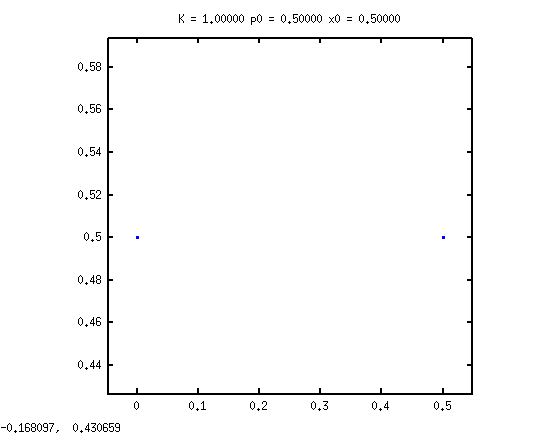
\includegraphics[width=.8\textwidth]{pointorbit.png}
\caption{Orbit plot of two points}
\label{pointorbit}
\end{figure}
\begin{figure}[H]
\centering
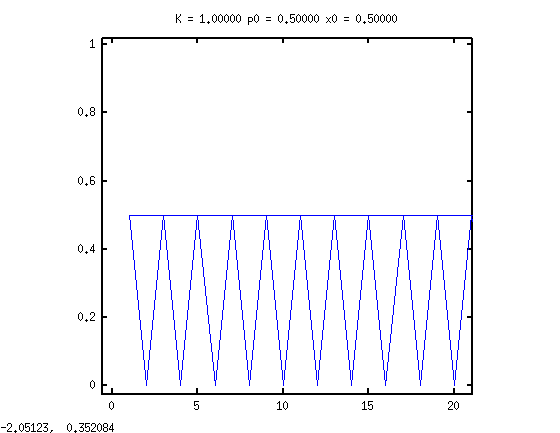
\includegraphics[width=.8\textwidth]{pointsvalues.png}
\caption{The values for $p$ and $x$ in the first steps }
\label{pointval}
\end{figure}

\subsection*{Curves}
\begin{figure}[H]
\centering
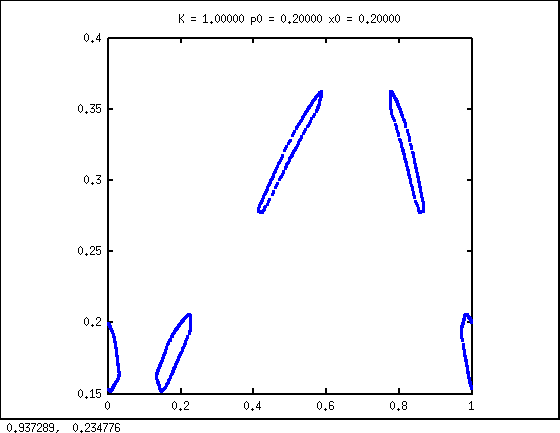
\includegraphics[width=.8\textwidth]{curvesorbit.png}
\caption{Orbit plot of four curves}
\label{curveorbit}
\end{figure}
\begin{figure}[H]
\centering
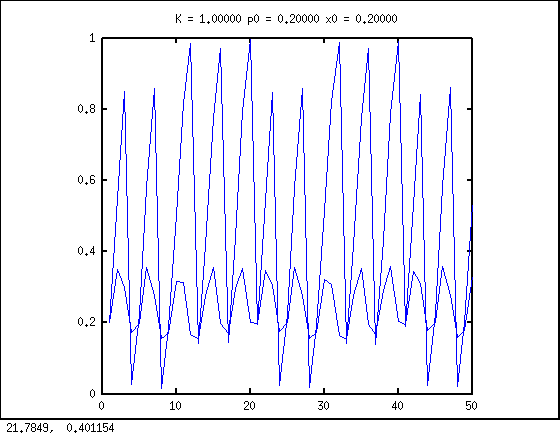
\includegraphics[width=.8\textwidth]{curvesvalues.png}
\caption{The values for $p$ and $x$ in the first steps }
\label{curveval}
\end{figure}

\newpage

In figure \ref{curveorbit} 4 curves. These curves are closed and symmetrical, which can be seen in the lower right and left side of the image.  The values of $p$ are between two range: a higher range, yielding the two top curves and a lower range, yielding the lower two curves. The value of $x$ varies between four ranges. In figure \ref{curveval} it can be seen that $x$ has a two different peak height at the top. The curves are visited in an fixed order as figure \ref{curveval} shows for the first few steps. Although the curve with $x$ values of 0.4 and 0.6 cannot be seen in this graph. It becomes clear that there are two alternating periods between the curves on the bottom and the top, in which the two lower curves are visited in an alternating order first. After a number of these periods, the two upper curves are visited in an alternating order.

\subsection*{Areas}
In figure \ref{areaorbit} two dotted areas can be seen. One on the top layer and one on the bottom. These areas seem to be symmetrical around the centre point of the image. These areas seem to be filled with chaotic values. In figure \ref{areaval} the values show peaks at the bottom and the top of the image, suggesting that the top area and the bottom area are visited in an alternating order.

\begin{figure}[H]
\centering
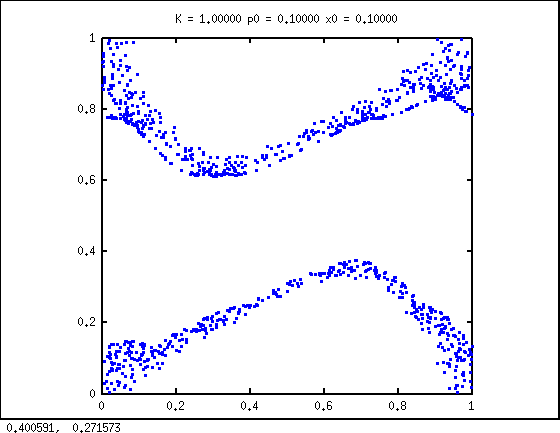
\includegraphics[width=.8\textwidth]{areaorbit.png}
\caption{Orbit plot of two areas}
\label{areaorbit}
\end{figure}

\newpage
\begin{figure}[H]
\centering
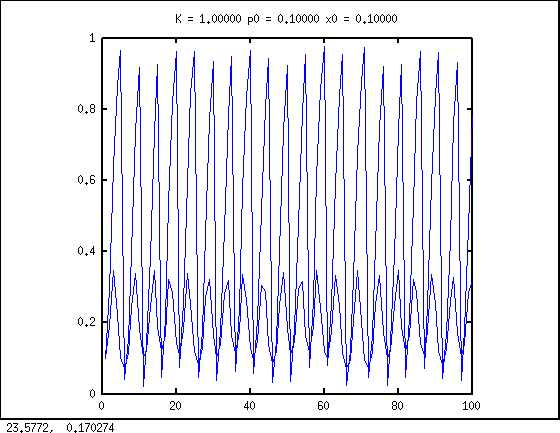
\includegraphics[width=.8\textwidth]{areavalues.png}
\caption{The values for $p$ and $x$ in the first steps }
\label{areaval}
\end{figure}

\subsection*{b) Behaviour for different values of $K$}

The figures 7 to 22 are taken at different values for $K$ in an increasing order.

\subsubsection*{Increasing value of $K$}
In figures 7 to 17 ($K$ values in the range of [0,1]) it can be seen that the straight lines at $K = 0$ slowly curve into two curves at the horizontal centre of the image. In between similar structures of curves visible.
Upward of $K = 0.9$ areas of chaotic dots appear and take up most of the image after $K = 2$, destroying the curves in the centre of the image.
After values of 3.0 for $K$ most of the area of the image is taken up by the chaotic region.\\
Around $K = 1.25$ six smaller curves can be seen on the edges of the two large centre curves. These become bigger and move outwards away from the centre of the large curve. When $K$ reaches a value of 2.0, these satellite curves are dissolved into the chaotic region of the image. This behaviour seems similar to the period doubling of the logistic map. For values of $K$ between 2.25 and 3.0, another instance of these smaller curves can be seen.

\subsubsection*{KAM orbits}
The lines displaying a KAM orbit are not very clearly visible, due to resolution errors. Instead the value 0.971635 as described by Greene\cite{kval} is used as the value for $K_c$. Figures 12 to 15 show plots of orbits for values of $K$ between 0.95 and 1.0. Although figures 14 and 15 show orbits spanning the entire interval of $[0,1]$, when zooming in, it becomes clear these do not follow a closed curve and are more of a chain of curves.

\begin{figure}[H]
\centering
\begin{minipage}{0.5\textwidth}
\centering
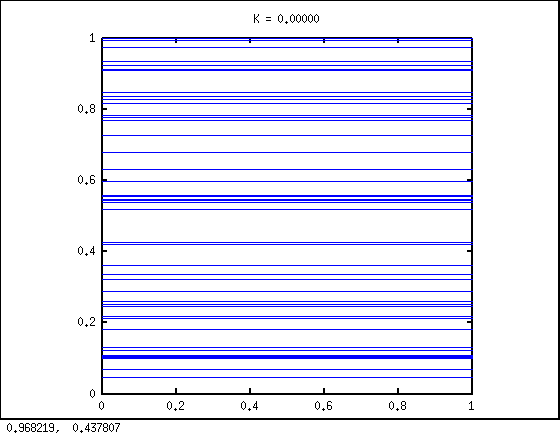
\includegraphics[width=\textwidth]{k0.png}
\caption{Orbits for $K = 0$}
\end{minipage}\hfill
\begin{minipage}{0.5\textwidth}
\centering
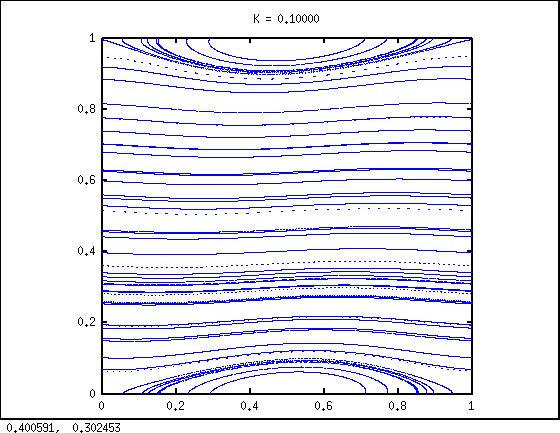
\includegraphics[width=\textwidth]{k01.png}
\caption{Orbits for $K = 0.1$}
\end{minipage}
\end{figure}

\begin{figure}[H]
\centering
\begin{minipage}{0.5\textwidth}
\centering
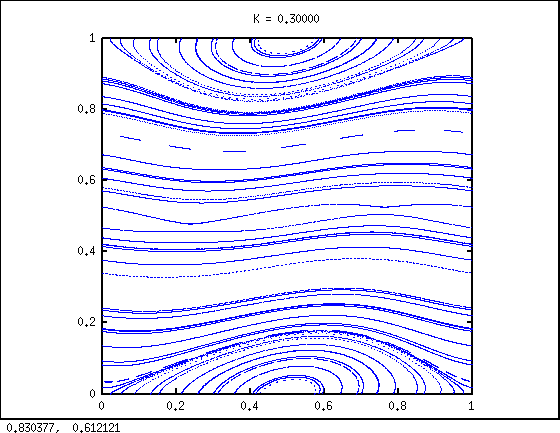
\includegraphics[width=\textwidth]{k03.png}
\caption{Orbits for $K = 0.3$}
\end{minipage}\hfill
\begin{minipage}{0.5\textwidth}
\centering
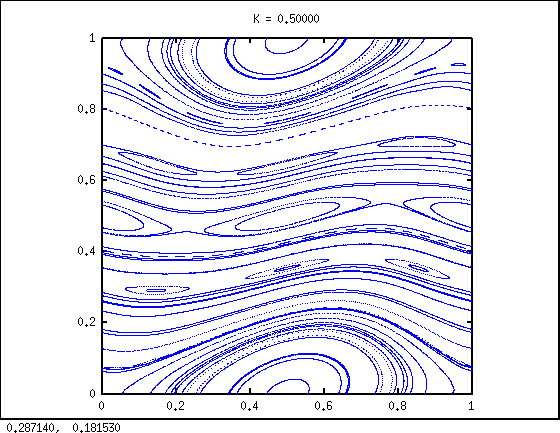
\includegraphics[width=\textwidth]{k05.png}
\caption{Orbits for $K = 0.5$}
\end{minipage}
\end{figure}

\begin{figure}[H]
\centering
\begin{minipage}{0.5\textwidth}
\centering
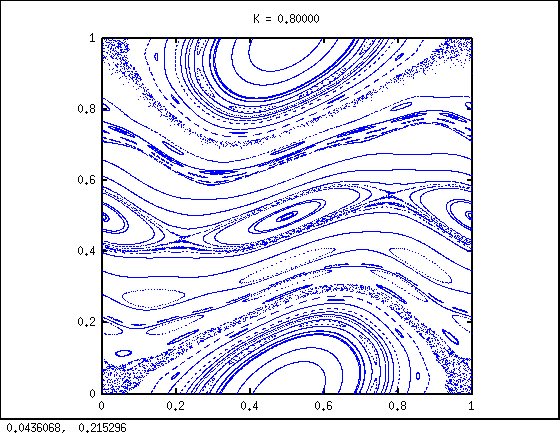
\includegraphics[width=\textwidth]{k08.png}
\caption{Orbits for $K = 0.8$}
\end{minipage}\hfill
\begin{minipage}{0.5\textwidth}
\centering
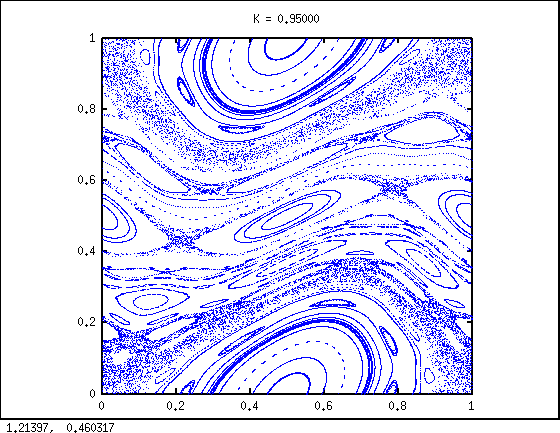
\includegraphics[width=\textwidth]{k095.png}
\caption{Orbits for $K = 0.95$}
\end{minipage}
\end{figure}

\begin{figure}[H]
\centering
\begin{minipage}{0.5\textwidth}
\centering
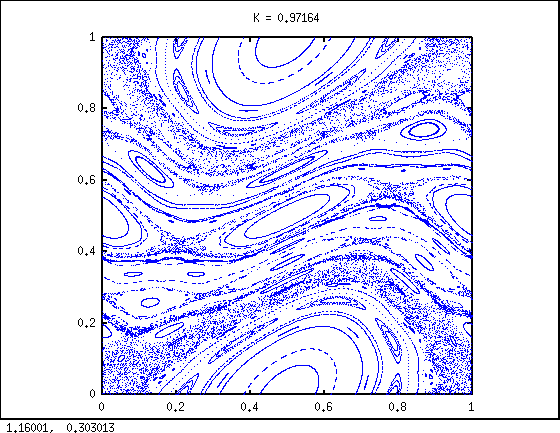
\includegraphics[width=\textwidth]{kc.png}
\caption{Orbits for $K_c = 0.97164$}
\end{minipage}\hfill
\begin{minipage}{0.5\textwidth}
\centering
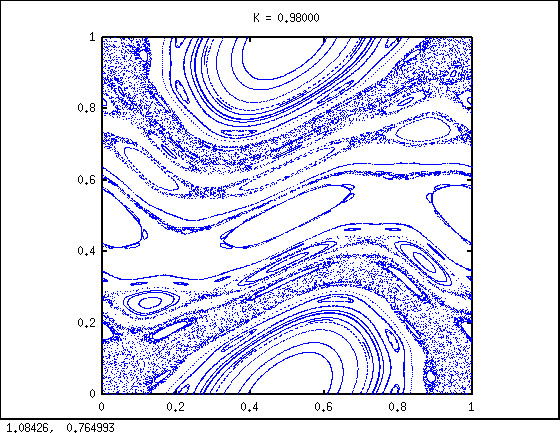
\includegraphics[width=\textwidth]{k098.png}
\caption{Orbits for $K = 0.98$}
\end{minipage}
\end{figure}

\begin{figure}[H]
\centering
\begin{minipage}{0.5\textwidth}
\centering
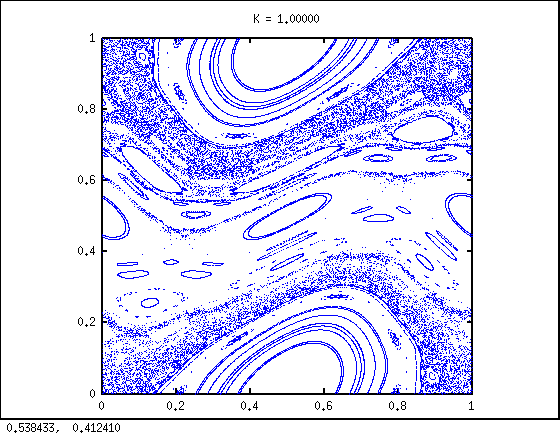
\includegraphics[width=\textwidth]{koneorbits.png}
\caption{Orbits for $K = 1.0$}
\end{minipage}\hfill
\begin{minipage}{0.5\textwidth}
\centering
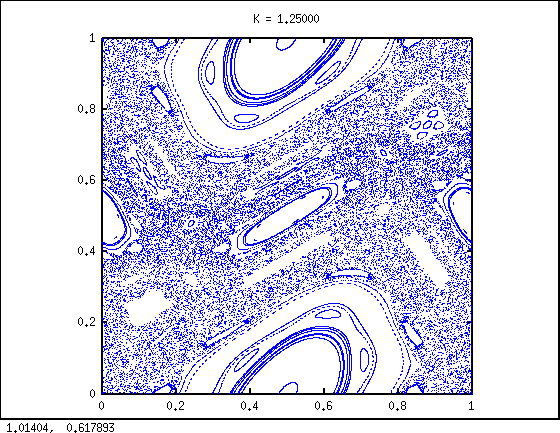
\includegraphics[width=\textwidth]{k125.png}
\caption{Orbits for $K = 1.25$}
\end{minipage}
\end{figure}

\begin{figure}[H]
\centering
\begin{minipage}{0.5\textwidth}
\centering
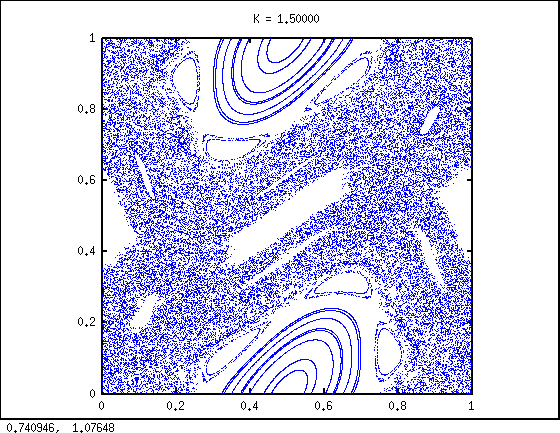
\includegraphics[width=\textwidth]{k15.png}
\caption{Orbits for $K = 1.5$}
\end{minipage}\hfill
\begin{minipage}{0.5\textwidth}
\centering
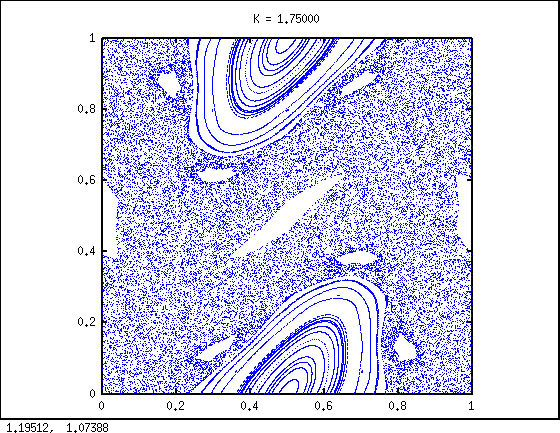
\includegraphics[width=\textwidth]{k175.png}
\caption{Orbits for $K = 1.75$}
\end{minipage}
\end{figure}

\begin{figure}[H]
\centering
\begin{minipage}{0.5\textwidth}
\centering
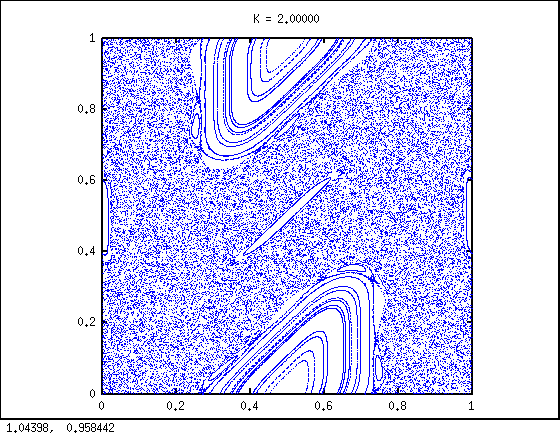
\includegraphics[width=\textwidth]{k20.png}
\caption{Orbits for $K = 2.0$}
\end{minipage}\hfill
\begin{minipage}{0.5\textwidth}
\centering
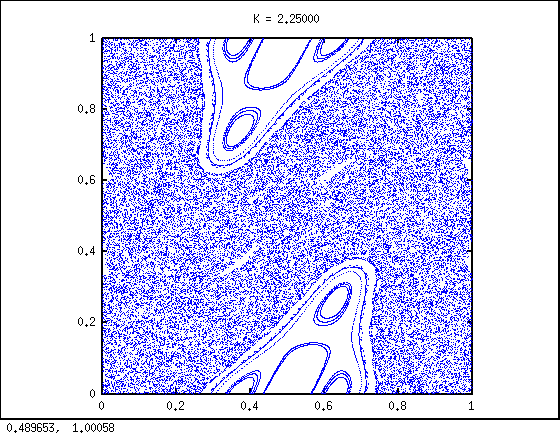
\includegraphics[width=\textwidth]{k225.png}
\caption{Orbits for $K = 2.25$}
\end{minipage}
\end{figure}

\begin{figure}[H]
\centering
\begin{minipage}{0.5\textwidth}
\centering
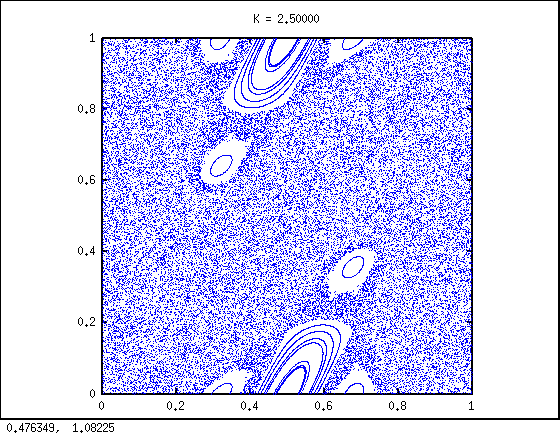
\includegraphics[width=\textwidth]{k25.png}
\caption{Orbits for $K = 2.5$}
\end{minipage}\hfill
\begin{minipage}{0.5\textwidth}
\centering
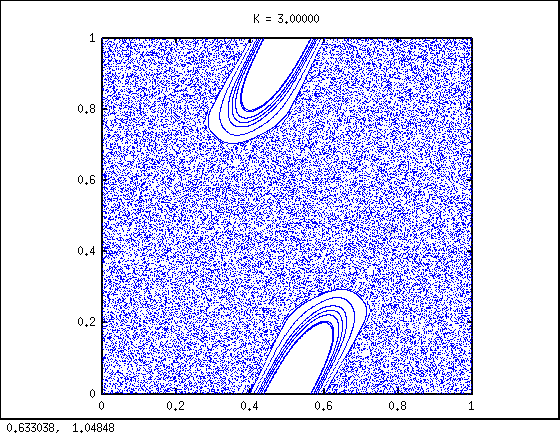
\includegraphics[width=\textwidth]{k30.png}
\caption{Orbits for $K = 3.0$}
\end{minipage}
\end{figure}

\section{Conclusion and discussion}

\subsection{a) 'Orbits' in the $x$-$p$ plane for fixed $K$}
From the different initial conditions three types of 'orbits' can be determined: Points, curves and areas. Each of these types has a certain order in which points are visited. For point orbits, these are clearly defined. For curves both values will vary in between ranges. For areas, the $x$ value will vary over the complete interval of $[0,1]$ and $p$ will vary only over smaller ranges.

\newpage

\subsection{b) Behaviour for different values of $K$}
For an increasing value of $K$ the amount of chaotic regions will increase. For values up to $K = 0.9$ the regions will be very small to non existent. After that the regions will grow. For values of $K$ in between $[1.0,1.75]$ and $[2.0,3.0]$ there will be a similar process to period doubling with smaller curves moving outward of the large centre curve. After $K = 3.0$ the image will only consist of the centre two curves and a chaotic region.\\
Exploring the limit of KAM orbits around the value of $K_c = 0.971635$ did not lead to observable results. Possibly to issues with the resolution of the plot and the amount of points per orbit plotted.

\subsection{Discussion}
Some of the images are not very clear. This is probably caused by the resolution at which they were taken. This is very visible in the example plots for $K_c$ where the plots of near $K$ values also show lines crossing the image completely horizontal. When zooming in on these lines, it becomes clear it has gaps in between evenly spaced dots. It is hard to prove from figures alone that a line could cross the entire horizontal scale of an image. Depending on the resolution and the amount of point generated for an orbit, this can change.\\
The plots of orbits for an increasing value of $K$ were generated by a pseudo-random number generator for the initial values. The random number generator was not seeded, so each image contains different orbits. The results would be more clear if each image was generated with the same initial values and $K$ being the only free variable.

\begin{thebibliography}{1337}
\bibitem{kval}
Greene, John M.\\
\emph{A method for determining a stochastic transition}\\
Journal of Mathematical Physics, 20, 1183-1201 (1979)\\ DOI:http://dx.doi.org/10.1063/1.524170

\end{thebibliography}
\end{document}
